% !TEX TS-program = pdflatex
% !TEX encoding = UTF-8 Unicode

% This is a simple template for a LaTeX document using the "article" class.
% See "book", "report", "letter" for other types of document.

\documentclass[11pt]{article} % use larger type; default would be 10pt

\usepackage[utf8]{inputenc} % set input encoding (not needed with XeLaTeX)

%%% Examples of Article customizations
% These packages are optional, depending whether you want the features they provide.
% See the LaTeX Companion or other references for full information.

%%% PAGE DIMENSIONS
\usepackage{geometry} % to change the page dimensions
\geometry{a4paper} % or letterpaper (US) or a5paper or....
% \geometry{margin=2in} % for example, change the margins to 2 inches all round
% \geometry{landscape} % set up the page for landscape
%   read geometry.pdf for detailed page layout information

\usepackage{graphicx} % support the \includegraphics command and options

% \usepackage[parfill]{parskip} % Activate to begin paragraphs with an empty line rather than an indent

%%% PACKAGES
\usepackage{booktabs} % for much better looking tables
\usepackage{array} % for better arrays (eg matrices) in maths
\usepackage{paralist} % very flexible & customisable lists (eg. enumerate/itemize, etc.)
\usepackage{verbatim} % adds environment for commenting out blocks of text & for better verbatim
\usepackage{subfig} % make it possible to include more than one captioned figure/table in a single float
\usepackage[export]{adjustbox} % center
\usepackage{hyperref}
\usepackage{float}
\usepackage[T1]{fontenc} %equal signs
\usepackage{amsmath} % summation notation
% These packages are all incorporated in the memoir class to one degree or another...

%%% HEADERS & FOOTERS
\usepackage{fancyhdr} % This should be set AFTER setting up the page geometry
\pagestyle{fancy} % options: empty , plain , fancy
\renewcommand{\headrulewidth}{0pt} % customise the layout...
\lhead{}\chead{}\rhead{}
\lfoot{}\cfoot{\thepage}\rfoot{}

%%% SECTION TITLE APPEARANCE
\usepackage{sectsty}
\allsectionsfont{\sffamily\mdseries\upshape} % (See the fntguide.pdf for font help)
% (This matches ConTeXt defaults)

%%% ToC (table of contents) APPEARANCE
\usepackage[nottoc,notlof,notlot]{tocbibind} % Put the bibliography in the ToC
\usepackage[titles,subfigure]{tocloft} % Alter the style of the Table of Contents
\renewcommand{\cftsecfont}{\rmfamily\mdseries\upshape}
\renewcommand{\cftsecpagefont}{\rmfamily\mdseries\upshape} % No bold!

%%% END Article customizations

%%% The "real" document content comes below...

\title{Can Money Buy Brains? \\
	\large A statistical analysis of Washington State teacher salaries and SAT scores}
\author{Ming Fong, Halle Hwang, Rae Gerking, Ethan Dang}
%\date{} % Activate to display a given date or no date (if empty),
         % otherwise the current date is printed 

\begin{document}
\maketitle

\section{Abstract}

It’s often said that \textit{money can't buy happiness}. Yet in today’s economic society, money seems to remain the driving factor in American lives, especially in the education system. While the United States remains the wealthiest nation in the world, it ranks 27th in healthcare and education, trailing behind a host of countries including Iceland, Finland, and the Netherlands. Furthermore, there has been a long debate in the American education system concerning teachers’ salaries and whether or not they are paid enough. To this day, many educators feel that they have been denied competitive, professional pay for too long and now, with 2018 being the biggest year of teacher strikes in this generation, the effects could have an impact on the performance of American students. In this retrospective study, we will observe these issues by researching and analyzing average teacher salaries throughout public high schools in Washington state and directly compare them with average student test scores from the respective schools. Our goal in this study is to determine whether or not there is a direct association between teacher salaries and student performance.

\section{Data Collection}

We collected our data using online government datasets that documented average SAT scores\footnote{SAT data: https://github.com/evilpegasus/APStats/blob/master/WA\%20\_District\_SAT\_2019.xlsx} by school district for the 2018-2019 school year, as well as the salary of every public-school teacher\footnote{ Salary data: https://github.com/evilpegasus/APStats/blob/master/WA\_School\_Personnel\_2018-2019.xlsx}. There are 208 data points for the state of Washington where both a district's mean SAT score and secondary teacher salaries were reported. Possible sources of bias include the fact that we only have salary data for public schools, some school districts did not report mean SAT scores and some teacher salaries may have been unreported. In order to draw the most accurate conclusion, we used a large dataset to counteract these biases. The original datasets can be found in the appendix.

\subsection{Data Processing}

With the raw salary data, all rows not containing a secondary teacher salary were filtered out and removed. Using a Python script, the secondary teacher salaries were read into a Pandas Dataframe, and the average of each district was found. To combine the datasets, the district names on the SAT dataset were renamed to match the naming convention of the salary spreadsheet. The renamed SAT dataset was then directly read into a Pandas Dataframe. The two Dataframes were merged by matching district names. Because not every district in the SAT dataset was listed on the salary dataset and not every salary district was listed on the SAT dataset, we only included districts with data from both sets.

\section{Analysis}

\subsection{Unit 1}

All statistical descriptions for both data sets were calculated with a computer. For the mean SAT data (see Figure 1), the distribution is roughly symmetric and unimodal. It is approximately normal-shaped. The median is at 1046.5 points and the mean is approximately 1043.995 points. The standard deviation is about 90.661 points. The minimum and maximum values are Taholah’s low mean score of 803 points and Mercer Island’s high mean score of 1316 points, which is an outlier (see Figure 2). The range is 513 points. The first quartile is 982 points and the third quartile is 1103.75 and the 1.5 * IQR is 182.625 points. This gives an upper fence of 1286.375 and a lower fence of 799.375. This confirms that Mercer Island’s mean score of 1316 is an outlier and Taholah’s mean of 803 points is not.

\begin{figure}[H]
  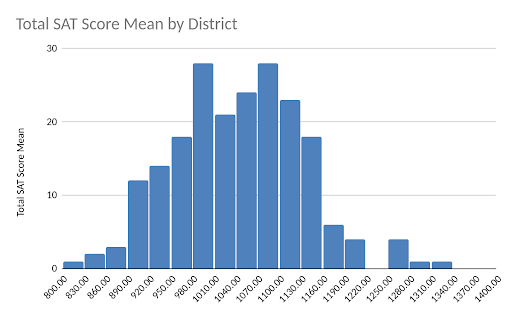
\includegraphics[scale=0.5,center]{figure1.png}
  \caption{Histogram}
  \label{fig:fig1}
\end{figure}
\begin{figure}[H]
  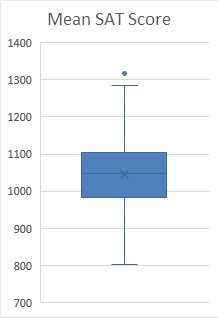
\includegraphics[scale=0.5,center]{figure2.png}
  \caption{Box and Whiskers Plot}
  \label{fig:fig2}
\end{figure}

For the average teacher salaries (see Figure 3), the data is multimodal and roughly symmetric and normal shaped. The mean is approximately \$80,040.33 and the median is \$80,158.9058. The standard deviation is about \$9,241.6781. There are two outliers, \$47,796.83333 (Coulee-Hartline) and \$107,466.3848 (Everett). The range is about \$59,669.5515. The first quartile is \$73,999.66 and the third quartile is \$85,988.53 and the 1.5 * IQR is \$17,983.3. The fences are \$56,016.36 and \$103,971.8 which confirms that Coulee-Hartline and Everett are indeed outliers (see Figure 4).

\begin{figure}[H]
  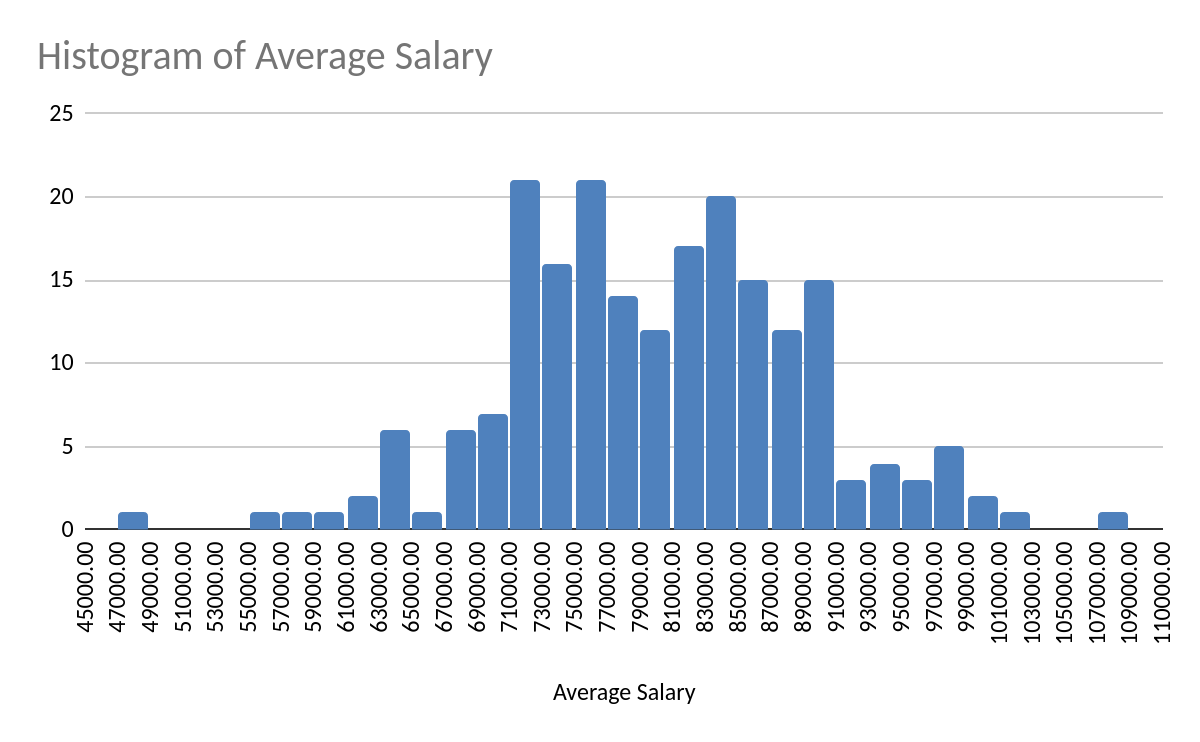
\includegraphics[scale=0.25,center]{figure3.png}
  \caption{Histogram}
  \label{fig:fig3}
\end{figure}
\begin{figure}[H]
  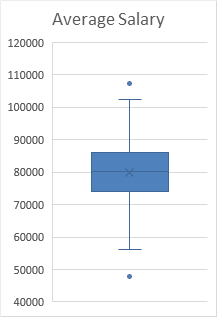
\includegraphics[scale=0.5,center]{figure4.png}
  \caption{Box and Whiskers Plot}
  \label{fig:fig4}
\end{figure}

\subsection{Unit 2}

Our scatter plot showed some positive correlation between teacher salary and mean SAT scores (see Figure 5). After plotting the residuals, we found the R\textsuperscript{2} value to be R\textsuperscript{2}=0.09423098779302452. This R\textsuperscript{2} value is small, but not negligible, and indicates that the linear relationship is weak. The R\textsuperscript{2} value tells us that the model accounts for approximately 9.42\% of the variance in average SAT scores by average teacher salaries. Some districts with interesting outliers in teacher salaries include Coulee-Hartline (\$47,796.83) and Everett (\$107,466.3848), the first district being a low outlier and the second being a high outlier. The district of Mercer Island (1316) is a high outlier in terms of average SAT score. Some lurking variables that might have adverse effects on our data and analysis include demographics, urban vs rural areas, and school district funding.  For instance, in urban areas, there are more opportunities to enroll in SAT prep programs or get private tutoring than in rural areas. Likewise, the demographics within each school affects the population’s abilities to further their SAT prep (through programs or tutoring) outside of school. School district funding positively correlates to SAT scores

\begin{figure}[H]
  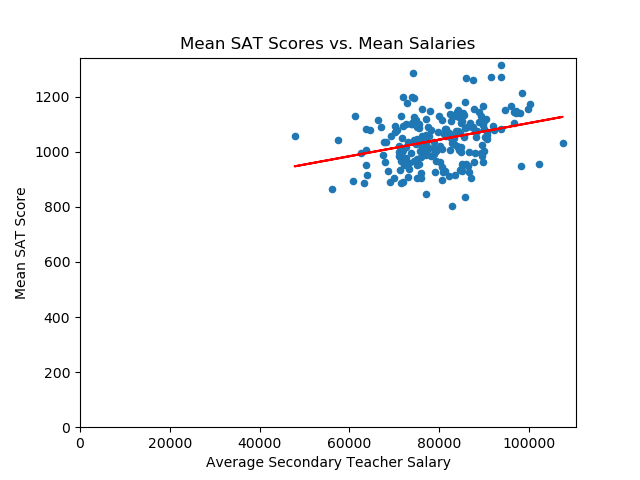
\includegraphics[scale=0.3,center]{figure5.png}
  \caption{Scatterplot and Linear Regression Line}
  \label{fig:fig4}
\end{figure}

Linear Regression Equation

\[\hat{y}=0.00301137x + 802.96409135\]

For each dollar increase in average secondary teacher salary, the mean SAT score of the district is predicted to increase by 0.00301137 points.

Our regression model predicts that a district paying teachers an average of \$0 will have a mean SAT score of 802.96409135. This situation is not realistic as no teacher would work for free. Additionally, a prediction at the y-intercept significantly extrapolates beyond our dataset: the lowest mean salary reported was \$47,796.83.

The R\textsuperscript{2} value and the regression equation coefficients were both computed with the Scikit-learn software library for Python.

\subsection{Unit 4}

The Renton School District has 91 secondary teachers with a 6-figure salary ($\geq$100000) out of a total of 295 secondary teachers. Given a simple random sample of 295 teachers from the set of all reported secondary teachers, what is the chance that more than 91 teachers are selected with six-figure salaries? There are 7234 secondary teachers in Washington State with six-figure salaries and 25511 total reported secondary teachers. 

We will use a binomial distribution to model this. We first check the conditions:

\[ np=82.610\geq10 \]
\[ nq=212.4\geq10 \]
\[ n=295<0.10*25511 \]

We can reasonably assume that most randomly selected salaries will be independent of each other. Using the binomial cumulative distribution function, we can find the probability that a random sample has equal to less than 91 teachers with six-figure salaries. The complement of that output will be our answer.

\[ \sum_{i=0}^{x} \binom{n}{i}(p)^i(1-p)^{n-1}=0.8447 \]
\[ 1-0.8447=0.1553 \]

Therefore, the probability that a randomly selected sample of 295 teachers has more than 91 teachers with a six-figure salary is 15.53\%. This means that the Renton School District has a relatively high concentration of high-earning secondary teachers.

\section{Conclusion}

This study focused on if teacher salaries and student performance have a direct association and the possible factors involved. From this study, we can conclude that there was a positive association between teacher salaries and student performance in SAT scores during the 2018-2019 school year. In context, if a district pays their secondary teachers more, their average SAT scores are likely to be higher.

The lurking variables that we theorized were demographics, urban vs rural areas, and school district funding, but it would be impractical to attempt to lessen the influence of these factors in our model. Similarly, another external factor is the variation in the cost of living between districts, which may have facilitated the differences in the demographics and teacher salaries of each school. For further research in the future, we could gather and use data from other states in the US similar to the data used in this study. We could also further consider the lurking factors stated above. Ultimately, our study exposed the flaws of the American education system and the unfair advantages wealth may give to students.

\section{Appendix}

WA Sat Scores: https://www.k12.wa.us/student-success/support-programs/dual-credit-programs/exam-based-dual-credit

\bigskip
\noindent WA Salary Data: https://www.k12.wa.us/safs-database-files

\bigskip
\noindent Repository of raw data, processed data, and analysis scripts: https://github.com/evilpegasus/apstats

\bigskip
\bigskip
\bigskip
\noindent The following pages contain the processed and combined data that was used in the analysis.
\end{document}
